\section{eo\-Invalidate\-Quad\-Op$<$ EOT $>$ Class Template Reference}
\label{classeo_invalidate_quad_op}\index{eoInvalidateQuadOp@{eoInvalidateQuadOp}}
One of the invalidator operators.  


{\tt \#include $<$eo\-Invalidate\-Ops.h$>$}

Inheritance diagram for eo\-Invalidate\-Quad\-Op$<$ EOT $>$::\begin{figure}[H]
\begin{center}
\leavevmode
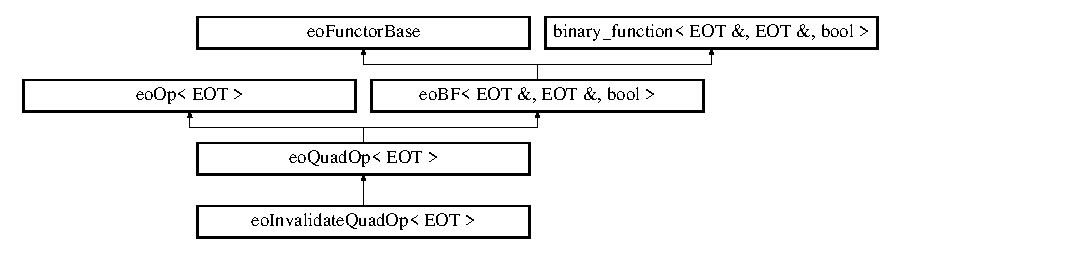
\includegraphics[height=2.96296cm]{classeo_invalidate_quad_op}
\end{center}
\end{figure}
\subsection*{Public Member Functions}
\begin{CompactItemize}
\item 
{\bf eo\-Invalidate\-Quad\-Op} ({\bf eo\-Quad\-Op}$<$ {\bf EOT} $>$ \&\_\-op)\label{classeo_invalidate_quad_op_a0}

\item 
bool {\bf operator()} ({\bf EOT} \&\_\-eo1, {\bf EOT} \&\_\-eo2)\label{classeo_invalidate_quad_op_a1}

\begin{CompactList}\small\item\em The pure virtual function that needs to be implemented by the subclass. \item\end{CompactList}\end{CompactItemize}
\subsection*{Private Attributes}
\begin{CompactItemize}
\item 
{\bf eo\-Quad\-Op}$<$ {\bf EOT} $>$ \& {\bf op}\label{classeo_invalidate_quad_op_r0}

\end{CompactItemize}


\subsection{Detailed Description}
\subsubsection*{template$<$class EOT$>$ class eo\-Invalidate\-Quad\-Op$<$ EOT $>$}

One of the invalidator operators. 

Use this one as a 'hat' on an operator that is defined to work on a generic datatype. This functor will then check the return type of the operator and invalidate the fitness of the individual.

This functor is used in algorithms that work with straight {\bf eo\-Mon\-Op}{\rm (p.\,\pageref{classeo_mon_op})}, {\bf eo\-Bin\-Op}{\rm (p.\,\pageref{classeo_bin_op})} or {\bf eo\-Quad\-Op}{\rm (p.\,\pageref{classeo_quad_op})} operators, for instance {\bf eo\-SGA}{\rm (p.\,\pageref{classeo_s_g_a})}. Note that {\bf eo\-Gen\-Op}{\rm (p.\,\pageref{classeo_gen_op})} derived operators generally do invalidate the fitness of the objects they have changed.

Return value means \char`\"{}Has\_\-Changed\char`\"{} and not \char`\"{}Needs\_\-To\_\-Be\_\-Invalidated\char`\"{} as successive invalidation are not really a problem 



Definition at line 114 of file eo\-Invalidate\-Ops.h.

The documentation for this class was generated from the following file:\begin{CompactItemize}
\item 
eo\-Invalidate\-Ops.h\end{CompactItemize}
